\chapter{对外兼容及安全防护}

从接口设计及安全防护的角度完善操作系统

\section{系统调用}

操作系统是用于管理硬件的软件,但是对绝大部分人都不算友好,
可友好不是操作系统必须的,操作系统只需要快速和高效,
为此操作系统向外界开放接口,
由其他的编程人员来使用接口完成各种功能的实现,
比如:图形界面,各种字处理软件等。

系统调用的实现是通过程序向操作系统申请权限访问各种指定的系统函数,
操作系统操作硬件完成工作。

向外界开发的系统调用接口:
\begin{enumerate}
    \item 显示单个字符
    \item 显示字符串
    \item 键盘输入
    \item 定时器
    \item 文件操作
    \item 命令行
\end{enumerate}

利用这些接口可以实现程序如下:
\begin{enumerate}
    \item 命令行计算器(调用键盘输入、显示字符串、命令行)
    \item 文本阅读器(调用文件操作)
    \item 音乐播放器(调用命令行、文件操作、定时器)
    \item 图片阅读器(调用命令行、文件操作)
\end{enumerate}

\subsection{命令行计算器}

    \subsubsection{预期设计}
        使用方法设计:calc+计算公式。 \\
        结果设计:分别以十进制和十六进制表示。

    \subsubsection{流程设计}
    命令行计算器的实现流程如图~\ref{fig:calc}所示。
        \begin{figure}[H]
            \centering
            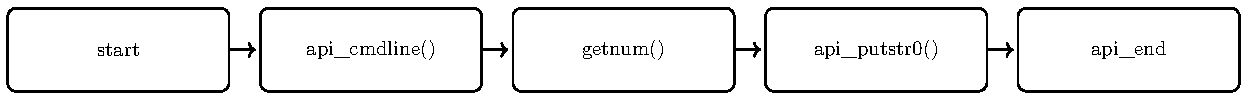
\includegraphics[width=\textwidth]{../Fig/api/calc.pdf}
            \caption{命令行计算器}
            \label{fig:calc}
        \end{figure}
        
        \csingle|int api_cmdline(char *buf, int maxsize);|
        \begin{itemize}
        \item 调用命令行系统接口
        \end{itemize}

        \csingle|int getnum(char **pp, int priority);|
        \begin{itemize}
        \item 获得数字与符号并计算
        \end{itemize}

        \csingle|void api_putstr0(char *s);|
        \begin{itemize}
        \item 输出运算结果
        \end{itemize}

        \csingle|void api_end(void);|
        \begin{itemize}
        \item 结束调用系统借口
        \end{itemize}

\subsection{文本阅读器}

    \subsubsection{预期设计}
        使用方法设计:tview+文本文件名。 \\
        结果设计:打开新窗口并显示文本内容。
    \subsubsection{实现过程}
    文本阅读器的实现流程如图~\ref{fig:tview}所示。
    % ../ZOS/src/apps/tview/tview.c

      \begin{figure}[H]
        \centering
        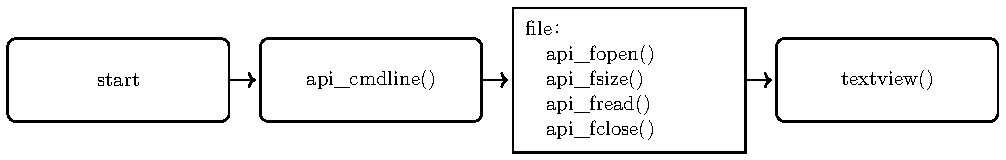
\includegraphics[width=\textwidth]{../Fig/api/tview.pdf}
        \caption{文本阅读器}
        \label{fig:tview}
      \end{figure}

    \csingle|api_fopen(char *fname);|
    \begin{itemize}
    \item 利用系统接口打开文件
    \end{itemize}
    
    \csingle|api_fsize(int fhandle, int mode);|
    \begin{itemize}
    \item 获取文件大小
    \end{itemize}

    \csingle|api_fread(char *buf, int maxsize, int fhandle);|
    \begin{itemize}
    \item 读取文件内容
    \end{itemize}

    \csingle|api_fclose(int fhandle);|
    \begin{itemize}
    \item 关闭文件
    \end{itemize}

    \csingle|textview(int win, int w, int h, int xskip, char *p, int tab, int lang)|
    \begin{itemize}
    \item 文件内容显示
    \end{itemize}

\subsection{音乐播放器}
    \subsubsection{预期设计}

    使用方法设计:mmlplay+歌曲文件名。

    结果设计:打开新窗口并播放音乐。
    \subsubsection{实现过程}
    音乐播放器的实现流程如图~\ref{fig:mmlplay}所示。
    \begin{figure}[H]
        \centering
        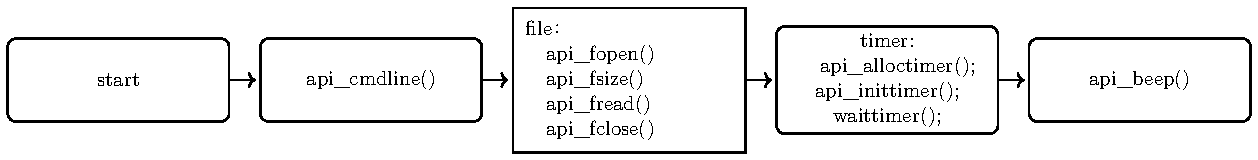
\includegraphics[width=\textwidth]{../Fig/api/mmlplay.pdf}
        \caption{音乐播放器}
        \label{fig:mmlplay}
      \end{figure}

    \csingle|api_alloctimer(void);|
    \begin{itemize}
    \item 分配定时器
    \end{itemize}

    \csingle|api_inittimer(int timer, int data);|
    \begin{itemize}
    \item 初始化定时器
    \end{itemize}

    \csingle|waittimer(int timer, int time);|
    \begin{itemize}
    \item 等待定时器
    \end{itemize}

    \csingle|api_beep(int tone);|
    \begin{itemize}
    \item 播放对应音符
    \end{itemize}

\subsection{图片阅读器}
    \subsubsection{预期设计}

    使用方法设计:gview+图片文件名。

    结果设计:打开新窗口并显示图片。
    \subsubsection{实现过程}
    图片阅读器的实现流程如图~\ref{fig:gview}所示。
    \begin{figure}[H]
        \centering
        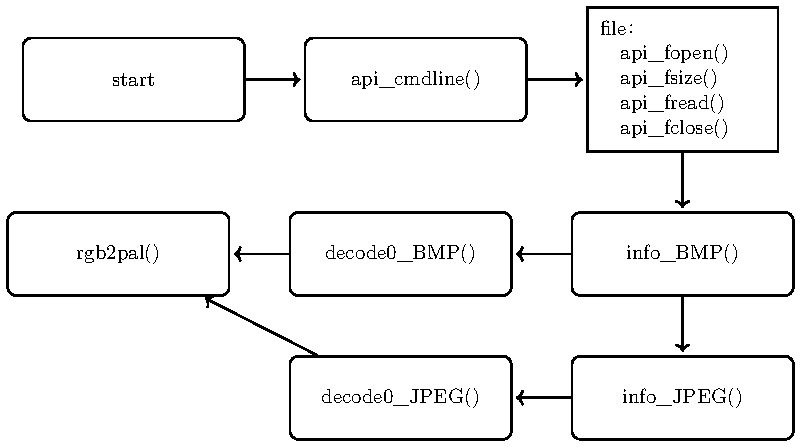
\includegraphics[width=.7\textwidth]{../Fig/api/gview.pdf}
        \caption{图片阅读器}
        \label{fig:gview}
      \end{figure}

    \csingle|info_BMP(struct DLL_STRPICENV *env, int *info, int size, char *fp);|
    \begin{itemize}
    \item 检查BMP文件信息
    \end{itemize}

    \csingle|info_JPEG(struct DLL_STRPICENV *env, int *info, int size, char *fp);|
    \begin{itemize}
    \item 检查JPG文件信息
    \end{itemize}

    \csingle|decode0_BMP(struct DLL_STRPICENV *env, int size, char *fp, int b_type, char *buf, int skip);|
    \begin{itemize}
    \item 解码BMP文件
    \end{itemize}

    \csingle|decode0_JPEG(struct DLL_STRPICENV *env, int size, char *fp, int b_type, char *buf, int skip);|
    \begin{itemize}
    \item 解码JPEG文件
    \end{itemize}

    \csingle|rgb2pal(int r, int g, int b, int x, int y);|
    \begin{itemize}
    \item 播放对应音符
    \end{itemize}

\section{系统安全}

只有完全封闭的系统才有可能成为真正安全的操作系统,但是既然选择了对外开放接口,
就必须重视外部应用程序的各种有意或无意的操作给操作系统带来的安全隐患,
一旦有程序跨越操作系统直接操作硬件很可能使得操作系统崩溃。

操作系统在开放接口的同时也需要一定的安全举措:
\begin{enumerate}
    \item 内存写保护:若将内存直接暴露给应用程序使得应用程序可能不慎在错误的地方写入错误的值,
    那么导致的问题可能包括系统崩溃、文件损坏,甚至导致计算机硬件损坏
    \item 系统函数权限:管理员的权限是通过各个系统函数实现的,将系统函数开放给对系统不熟悉的用户是完全不负责任的)
    \item 监测并终端异常程序:计算机病毒是自发的运行并对计算机造成意想不到后果的恶意程序,
    所以在操作系统发现有程序活动异常时应该立即中断此程序
    \item 系统调用防护:系统调用的目的是使得外部开发者通过系统设计者的意愿得到希望得到的系统函数执行权而开发应用程序,
    于是在系统调用方面,每一个系统调用接口都应该绑定固定的系统函数,并限制其用法,拒绝非系统调用的方式启用系统函数。
\end{enumerate}